\documentclass{beamer}
%
% Choose how your presentation looks.
%
% For more themes, color themes and font themes, see:
% http://deic.uab.es/~iblanes/beamer_gallery/index_by_theme.html
%
\mode<presentation>
{
  \usetheme{Warsaw}      % or try Darmstadt, Madrid, Warsaw, ...
  \usecolortheme{default}
  \usepackage{beamerthemesplit}% or try albatross, beaver, crane, ...
  \usefonttheme{structurebold}  % or try serif, structurebold, ...
  \setbeamertemplate{navigation symbols}{}
  \setbeamertemplate{caption}[numbered]
  
} 

\usepackage[english]{babel}
\usepackage[utf8x]{inputenc}
\usepackage{amsmath,amssymb}
\usepackage[absolute,overlay]{textpos}
\usepackage{graphicx} 
\logo{
\includegraphics[height=0.75cm]{images/Logo_Universita_Milano-Bicocca.jpg}}
\title[Schema-Linking \hspace{0.5cm}\insertframenumber/\inserttotalframenumber]{Schema Linking}
\author{Juan Carlos Rosito Cuellar}
\institute{Universita' degli studi di Milano-Bicocca}
\date{16-4-2019}

\usepackage{caption}
\DeclareCaptionFont{xxviii}{\fontsize{7}{7}\selectfont}
\captionsetup{font=xxviii}
\newcommand\Fontvi{\fontsize{6}{9}\selectfont}

%%%%%%%%%%%%%%% IMPORT FORM DOCUMENT %%%%%%%%%%%%%%%%%%%%%%%%%%%
%\documentclass{llncs}
\usepackage{graphicx}
\usepackage{xargs}
%\usepackage[pdftex,dvipsnames]{xcolor}
\usepackage{amsmath}
\usepackage[]{algorithm2e}
\usepackage{amsfonts}
\usepackage{mathtools}
\DeclareMathOperator*{\argmin}{arg\,min}
\DeclareMathOperator*{\argmax}{arg\,max}

%TODO PACKAGE
\usepackage[colorinlistoftodos,prependcaption,textsize=tiny]{todonotes}
\newcommandx{\unsure}[2][1=]{\todo[linecolor=red,backgroundcolor=red!25,bordercolor=red,#1]{#2}}
\newcommandx{\change}[2][1=]{\todo[linecolor=blue,backgroundcolor=blue!25,bordercolor=blue,#1]{#2}}
\newcommandx{\info}[2][1=]{\todo[linecolor=OliveGreen,backgroundcolor=OliveGreen!25,bordercolor=OliveGreen,#1]{#2}}
\newcommandx{\improvement}[2][1=]{\todo[linecolor=Plum,backgroundcolor=Plum!25,bordercolor=Plum,#1]{#2}}
\newcommandx{\thiswillnotshow}[2][1=]{\todo[disable,#1]{#2}}





\begin{document}


\begin{frame}
	\titlepage
\end{frame}


%\section{Introduction}
\begin{frame}{The scope of the challenge}
	Semantic Web Challenge on Tabular Data to Knowledge Graph Matching
	\begin{itemize}
		\item Tabular data in the form of CSV files is the common input format in a data analytics pipeline. However a lack of understanding of the semantic structure and meaning of the content may hinder the data analytics process. Thus gaining this semantic understanding will be very valuable for data integration, data cleaning, data mining, machine learning and knowledge discovery tasks.
		\item This challenge aims at benchmarking systems dealing with the tabular data to KG matching problem, so as to facilitate their comparison on the same basis and the reproducibility of the results.
	\end{itemize}
\end{frame}

\begin{frame}{objectives}
	\begin{itemize}
		\item Recommend a schema semantical annotation of a table
		      \begin{itemize}
			      \item Get Type Candidates based on the instances of the table
			      \item Get Predicate Candidates based on the Types of each Column of the table
			      \item Generate a Score of all Types and Columns
			      \item Generate all possible Ontologies with the candidates of Type and Predicate.
			      \item Generate a Score of all possible Ontologies.
			      \item Choose the best Schema semantical annotation of the Table
		      \end{itemize}
	\end{itemize}

\end{frame}



\begin{frame}{Introduction: Definitions}
	\begin{figure}
		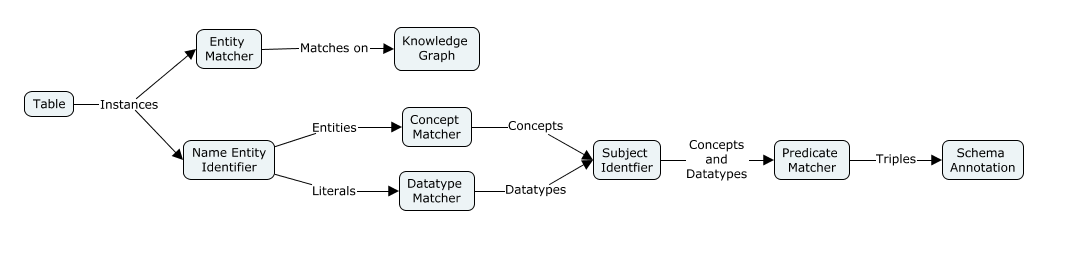
\includegraphics[width=11cm]{images/Formalization_diagram.png}
		\caption{\label{fig:your-figure2} Tabular overview of the variables}
	\end{figure}
\end{frame}

\begin{frame}{The inputs of table interpretation: TABLE}
	\begin{definition}[Table]
		We define \textit{Table} a rectangular array (matrix) of strings arranged in $n$ rows and $m$ columns. Every pair $(i,j)$ with $1\leq i \leq n$ and $1\leq j \leq m$, is unambiguously identifies a \textit{cell} of the table.
	\end{definition}

	\begin{definition}[Rows and Columns]
		Given an $n\times m$ table, let $r_i$ denote the i-th row of the table, that is $r_i =\{(i,j) | 1\leq j \leq m\}$ and  $c_j$ denote the j-th column ($c_j =\{(i,j) |1\leq i \leq n\}$).
		Let $\mathcal{R} = \{r_i | 1\leq j \leq m\}$ and $\mathcal{C} = \{c_j|1\leq i \leq n\}$ be the set of all rows and columns of the table, respectively.
	\end{definition}
\end{frame}

\begin{frame}{The inputs of table interpretation: TABLE2}
	\begin{definition}[Column header function]
		A Column Header Function $h: \mathcal{C}\to \mathcal{L}$ associates each column with a word of a language $\mathcal{L}$.
	\end{definition}

	\begin{definition}[Header Table]
		We define a Header Table the pair $T_h =(T, h)$ where  $T$ is a table and h is a column header function.
	\end{definition}

	\begin{definition}[Header]
		Given a header table $T_h =(T, h)$, we define $\mathcal{H}=h(\mathcal{C})$ as the header of table T.
	\end{definition}
\end{frame}


\begin{frame}{The inputs of table interpretation: Semantic}
	\begin{definition}[Ontology - simplified definition]
		An ontology is a multigraph
		$\mathcal{O}=(\mathcal{N}, \mathcal{P}, \mathcal{A})$, where:
		\begin{itemize}
			\item $\mathcal{N} =\mathcal{N}_c \cup \mathcal{N}_d$ is the set of the entities in $\mathcal{O}$ (e.g., {DBpedia Ontology, GeoNames Ontology, ...})
			      \begin{itemize}
				      \item $\mathcal{N}_c$ is the set of concepts (e.g., {dbo:Movie, dbo:Actor, ...})
				      \item $\mathcal{N}_d$ is the set of data types (e.g., {xsd:date, xsd:integer, ...})
			      \end{itemize}
			\item $\mathcal{P}$ is the property label set (e.g., {“starring”, “releaseDate”, ...})
			\item $\mathcal{A} \subset \mathcal{N}^2\times\mathcal{P}$ set of labeled directed arcs, where an edge can exist only between concepts or between a concept and a data type.
		\end{itemize}
	\end{definition}
\end{frame}


\begin{frame}{The inputs of table interpretation: Semantic 2}
	\begin{definition} [Knowledge Graph]
		Given an ontology $\mathcal{O}=(\mathcal{N},\mathcal{P}, \mathcal{A})$,
		a \textit{Knowledge Graph} $\mathcal{KG}$ \cite{SHI2016123} is a directed multigraph defined by the tuple
		$\mathcal{KG}=(\mathcal{V, E, O}, \psi, \phi)$ where:
		\begin{itemize}
			\item $\mathcal{V}$ is the set of vertices; a vertex represents an entity or a literal (e.g., {dbr:The Matrix, dbr:Keanu Reeves, "1999", ...})
			\item $\mathcal{E} \subset \mathcal{V}^2$ is a set of directed edges connecting two nodes, they represent links between two entities;
			\item $\psi$ is the ontology mapping function $\psi:\mathcal{V}\to \mathcal{N}_o$, which links an entity vertex to a concept or data type in the ontology (e.g., dbo:Movie links dbr:The Matrix, dbo:Actor links dbr:Keanu Reeves, xsd:date links “1999”)
			\item $\phi$ is the predicate mapping function $\phi:\mathcal{E} \to \mathcal{E}$, which maps an edge to a predicate type (e.g. dbr:The Matrix dbo:starring dbr:Keanu Reeves, dbr:The Matrix dbo:releaseDate “1999”).
		\end{itemize}
	\end{definition}
\end{frame}




\begin{frame}{The inputs of table interpretation: Formalization}
	Given an $m\times n$ header table $\mathcal{T} =(T, h)$:
	\begin{itemize}
		\item $T = \{t_{ij}: 1\leq i \leq n \land  1\leq j \leq m\}$ where $t_{ij}$ is the element contained in the cell $(i, j)$
		\item $\mathcal{C} = \{c_1,...,c_m\}$ where $c_j$ is the j-th column
		\item $\mathcal{R} = \{r_1,...,r_n\}$ where $r_i$ is the i-th row
	\end{itemize}
	And a \textit{set of Knowledge Graphs} $\mathcal{KG}$s is defined as follows:\\
	$\mathcal{KG}s = \{\mathcal{KG}_1,\mathcal{KG}_2,\ldots,\mathcal{KG}_k\}$\\

\end{frame}


\begin{frame}{The inputs of table interpretation: Formalization2}
	And a \textit{Knowledge Graph} $\mathcal{KG}$, defined as follows:\\
	$\mathcal{KG}_x=(\mathcal{V}_x, \mathcal{E}_x, \mathcal{O}_x, \psi_x, \phi_x)$
	\begin{itemize}
		\item $\mathcal{V}_x =\mathcal{Z}_x\cup\mathcal{L}_x $
		      \begin{itemize}
			      \item $\mathcal{Z}_x$ is a set of entities in the $\mathcal{KG}_x$
			      \item $\mathcal{L}_x$ is a set of literals
		      \end{itemize}
		\item $\mathcal{E}_x$ is a set of labeled directed edges between two elements in $\mathcal{N}_x$
		      %\item $\mathcal{P}_x$ is a set of property label in $\mathcal{KG}_x$
		\item $\mathcal{O}_x =(\mathcal{N}_x,\mathcal{P}_x, \mathcal{A}_x)$ with $\mathcal{N}_x = \mathcal{N}_{cx} \cup \mathcal{N}_{dx}$
		      \begin{itemize}
			      \item $\mathcal{N}_{cx}$ is a set of concepts in the $\mathcal{KG}_x$
			      \item $\mathcal{N}_{dx}$ is a set of datatypes in the $\mathcal{KG}_x$
		      \end{itemize}
		\item $\psi_x: \mathcal{V}_x\to \mathcal{N}_x$ is the ontology mapping function
		\item $\phi_x: \mathcal{E}_x\to\mathcal{A}_x$ is the predicate mapping function
	\end{itemize}
\end{frame}


\begin{frame}{The inputs of table interpretation: Concept}
	\begin{definition}[Concept Matcher]
		Given a knowledge base $\mathcal{KG}_x$, the \textit{Concept Matcher} is a function $\theta_x: T \to \mathcal{N}_{cx} \cup \emptyset$:
		\begin{equation}
			\eta_x(t_{ij})=
			\begin{cases}
				c\in\mathcal{N}_{cx}
				\\
				\emptyset
			\end{cases}
			\forall t_{ij} \in T
		\end{equation}
	\end{definition}
\end{frame}


\begin{frame}{The inputs of table interpretation: Type}
	\begin{definition}[Datatype Matcher]
		Given a knowledge base $\mathcal{KG}_x$, the \textit{Datatype Matcher} is a function $\theta_x: T \to \mathcal{N}_{dx} \cup \emptyset$:
		\begin{equation}
			\theta_x(t_{ij})=
			\begin{cases}
				d\in\mathcal{N}_{dx}
				\\
				\emptyset
			\end{cases}
			\forall t_{ij} \in T
		\end{equation}
	\end{definition}
\end{frame}


\begin{frame}{The inputs of table interpretation: Type}
	\begin{definition}[Entity Matcher] Given a knowledge base $\mathcal{KG}_x$, an \textit{Entity Matcher} is a function $\chi_x: T \to \mathcal{Z}_x \cup \emptyset$:
		\begin{equation}
			\chi_x(t_{ij})=
			\begin{cases}
				z\in\mathcal{Z}_x
				\\
				\emptyset
			\end{cases}
			\forall t_{ij} \in T
		\end{equation}
	\end{definition}
\end{frame}


\usetikzlibrary{arrows,automata}

\begin{frame}{The inputs of table interpretation: Type2}
	\begin{lemma} Given a knowledge base $\mathcal{KG}_x$ and an \textit{Entity Matcher} is a function $\chi_x$, a particular Concept Matcher is defined as:
		\begin{equation}
			\eta_x(t_{ij})=
			\begin{cases}
				\psi_x(\chi_x(t_{i,j})), & if~ \chi_x(t_{i,j})\in \mathcal{Z}_x
				\\
				\emptyset,               & otherwise
			\end{cases}
			~\forall t_{ij} \in T
		\end{equation}
	\end{lemma}
	\begin{tikzpicture}[->,>=stealth',shorten >=1pt,auto,node distance=2.8cm,
			semithick]
		\tikzstyle{every state}=[fill=white,draw=black,text=black]

		\node[state] (A){$t_{ij}\in T$};
		\node[state] (B) [right of=A] {$z\in \mathcal{Z}_x$};
		\node[state] (C) [ right of=B] {$c\in \mathcal{N}_{cx}$};

		\path (A) edge   node {$\chi_x$} (B)
		(B) edge   node {$\psi_x$} (C);
	\end{tikzpicture}
\end{frame}


\begin{frame}{The inputs of table interpretation: Entity Identifier}
	\begin{definition}[Name Entity Identifier]
		Given a knowledge base $\mathcal{KG}_x$, a \textit{Name Entity Identifier} is function $\alpha_x: \mathcal{C}\to \{\text{``Name Entity''}, \text{``Literal''} \}$.
	\end{definition}

	\begin{lemma}
		Given a knowledge base $\mathcal{KG}_x$, a threshold value $\bar{\gamma}\in \mathbb{R}$, and a function $\beta_x: T \to \{1,0\}$ defined as follows:
		\begin{equation}
			\beta_x(t_{ij})=
			\begin{dcases}
				1, & if~  \eta_x(t_{i,j}) \in\mathcal{N}_{cx}
				\\
				0, & ~ otherwise
			\end{dcases}
		\end{equation}
		a particular \textit{Name Entity Identifier} can be defined as:
		\begin{equation}
			\alpha_x(c_{j})=
			\begin{dcases*}
				\text{``Name Entity''}, & if  $\sum_i \beta_x(t_{ij})\geq\bar{\gamma}$;
				\\
				\text{``Literal''}, & otherwise.
			\end{dcases*}
			\ \ \forall c_j \in \mathcal{C}
		\end{equation}
	\end{lemma}
\end{frame}


\begin{frame}{The inputs of table interpretation: Subject Identifier}
	\begin{definition}[Subject Identifier]
		Given a knowledge base $\mathcal{KG}_x$, an $m\times n$ header table $\mathcal{T} =(T, h)$: we define \textit{Subject Identifier} a function $\sigma_x: \mathcal{T} \to \{1, 0\}^m$ so that $\displaystyle\sum^m_{j=1} \sigma_x(\mathcal{T})_j =1$ and $\sigma_x(\mathcal{T})_j = 0,~\forall j\in \{j | \alpha_x(c_j) =1\}$.
	\end{definition}
\end{frame}


\begin{frame}{The inputs of table interpretation: Semantic Column Annotator}
	\begin{definition}[Semantic Column Annotator]
		Given a knowledge base $\mathcal{KG}_x$, a table defined by a set of columns $\mathcal{C}$ a Semantic Column Annotator is a function $\zeta_x: \mathcal{C}\to \mathcal{N}_x$.
	\end{definition}
\end{frame}


\begin{frame}{The inputs of table interpretation: Semantic Column Annotator 2}
	\begin{lemma}
		Given a knowledge base $\mathcal{KG}_x$, a table T, a concept matcher $\eta_x$, a datatype matcher $\theta_x$, and sets $\mathcal{D}^j_{cx}$ and $\mathcal{D}^j_{dx}$ defined as follows:
		\begin{align*}
			\mathcal{D}^j_{cx} & =\{t_{ij} | t_{ij}\in T \wedge\eta_x(t_{ij}) =cx \wedge i \in \{i,\ldots, n\}\},    & \forall cx \in \mathcal{N}_{cx} \wedge \forall j \in \{1,\ldots,m\} \\
			\mathcal{D}^j_{dx} & =\{t_{ij} | t_{ij}\in T \wedge \theta_x(t_{ij}) =dx \wedge i \in \{i,\ldots, n\}\}, & \forall dx \in \mathcal{N}_{dx} \wedge \forall j \in \{1,\ldots,m\}
		\end{align*}
		The function:
		\begin{equation}
			\zeta(c_{j})=
			\begin{dcases*}
				\argmax_{c_x\in \mathcal{N}_{cx}}|D^j_{cx,}|, & if $\alpha(c_{j})=1$;
				\\
				\argmax_{d_x\in \mathcal{N}_{dx}}|\mathcal{D}^j_{dx}|,& otherwise.
			\end{dcases*}
		\end{equation}
		is a Semantic Column Annotator.
	\end{lemma}
\end{frame}

\begin{frame}{The inputs of table interpretation: Predicate Matcher}

	\begin{definition}[Predicate Matcher]
		$\pi_x:\mathcal{C}^2\to \mathcal{A}_x\cup \emptyset$ with $\pi_x(c_i,c_j) =\emptyset,\, \forall (i,j)| i=j$.
	\end{definition}
\end{frame}


\begin{frame}{Methodology: Pipe-Line}
	\begin{figure}
		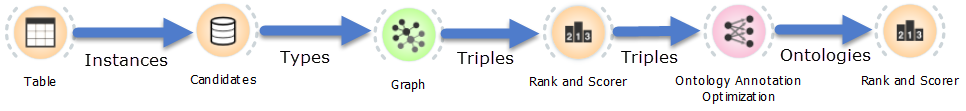
\includegraphics[width=10cm]{images/diagrams2.png}
		\caption{\label{fig:your-figure2} Fluid Diagram of the Schema annotation}
	\end{figure}
\end{frame}

\begin{frame}{Methodology: Pipe-Line 2}
	\begin{figure}
		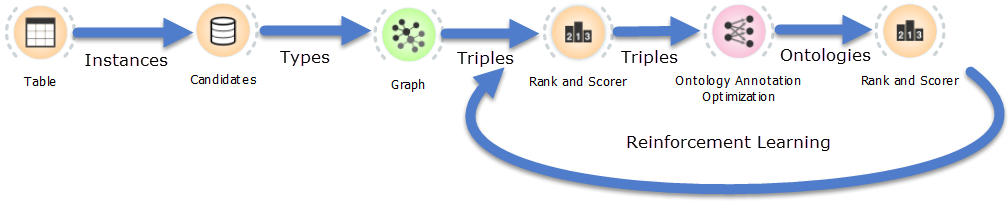
\includegraphics[width=11cm]{images/diagrams.png}
		\caption{\label{fig:your-figure2} Fluid Diagram of the Schema annotation with the implementation of Reinforcement Learning}
	\end{figure}
\end{frame}

% 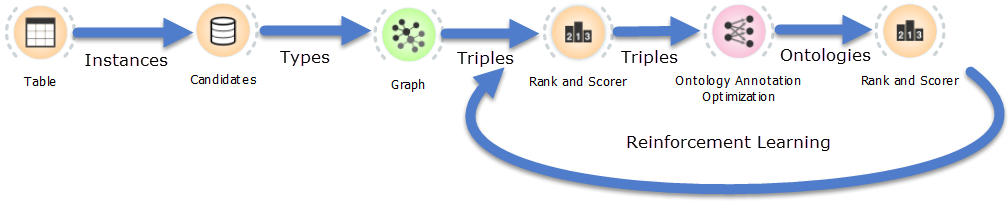
\includegraphics[height=1cm,width=0.5cm]{images/diagrams.png}
% \addtobeamertemplate{frametitle}{}{%
% \begin{textblock*}{100mm}(.85\textwidth,-1cm)
% 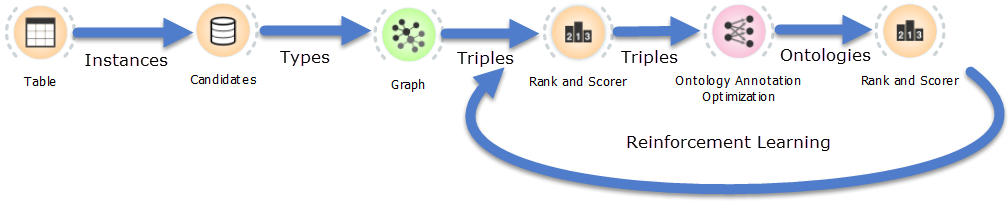
\includegraphics[height=1cm,width=2cm]{images/diagrams.png}
% \end{textblock*}}





\begin{frame}{Methodology: Candidate - 1}
	\begin{textblock*}{4cm}(8.5cm,0.05cm) % {block width} (coords)
		
\includegraphics[width=4cm]{images/header-candidate.png}
	\end{textblock*}
	\begin{figure}
		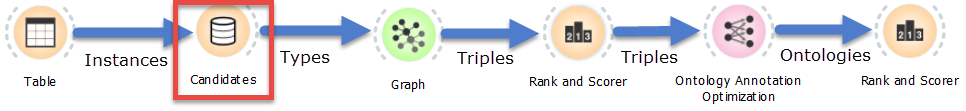
\includegraphics[width=10cm]{images/diagrams-candidate.png}
		%\caption{\label{fig:your-figure2} TableMiner design by Z.Zhang}
	\end{figure}
\end{frame}
\begin{frame}{Methodology: Candidate - 2}
	\begin{textblock*}{4cm}(8.5cm,0.05cm) % {block width} (coords)
		
\includegraphics[width=4cm]{images/header-candidate.png}
	\end{textblock*}
	\begin{definition}[Type Candidate Maker]
		datto SPARQL
	\end{definition}
\end{frame}
\begin{frame}{Methodology: Candidate - 3}
	\begin{textblock*}{4cm}(8.5cm,0.05cm) % {block width} (coords)
		
\includegraphics[width=4cm]{images/header-candidate.png}
	\end{textblock*}
	State of art
	\begin{itemize}
		\item SPARQL
		\item LOD TermPicker
		\item LOV
		\item Cod-start disambiguation TableMiner
	\end{itemize}
\end{frame}
\begin{frame}{Methodology: Candidate - 4}
	\begin{textblock*}{4cm}(8.5cm,0.05cm) % {block width} (coords)
		
\includegraphics[width=4cm]{images/header-candidate.png}
	\end{textblock*}
	Scoring
	\begin{itemize}
		\item SPARQL
		\begin{itemize}
			\item Counting Number of instances of each Type for each column
		\end{itemize}
	\end{itemize}
\end{frame}



\begin{frame}{Methodology: Graph - 1}
	\begin{textblock*}{4cm}(8.5cm,0.05cm) % {block width} (coords)
		
\includegraphics[width=4cm]{images/header-graph.png}
	\end{textblock*}
	\begin{figure}
		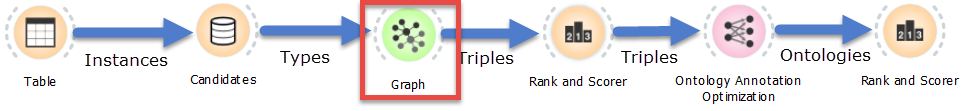
\includegraphics[width=10cm]{images/diagrams-graph.png}
		%\caption{\label{fig:your-figure2} TableMiner design by Z.Zhang}
	\end{figure}
\end{frame}
\begin{frame}{Methodology: Graph - 2}
	\begin{textblock*}{4cm}(8.5cm,0.05cm) % {block width} (coords)
		
\includegraphics[width=4cm]{images/header-graph.png}
	\end{textblock*}
	\begin{definition}[Predicate Candidate]
		datto ABSTAT
	\end{definition}
\end{frame}
\begin{frame}{Methodology: Graph - 3}
	\begin{textblock*}{4cm}(8.5cm,0.05cm) % {block width} (coords)
		
\includegraphics[width=4cm]{images/header-graph.png}
	\end{textblock*}
	State-of-the-Art
	\begin{itemize}
		\item ABSTAT
		\item Relation Enumeration/Literal column annoatation - Table Miner
	\end{itemize}
\end{frame}
\begin{frame}{Methodology: Graph - 4}
	\begin{textblock*}{4cm}(8.5cm,0.05cm) % {block width} (coords)
		
\includegraphics[width=4cm]{images/header-graph.png}
	\end{textblock*}
	Scoring
	\begin{itemize}
		\item Frequency ABSTAT
	\end{itemize}
\end{frame}


\begin{frame}{Methodology: Ranking Triples - 1}
	\begin{textblock*}{4cm}(8.5cm,0.05cm) % {block width} (coords)
		
\includegraphics[width=4cm]{images/header-rank-triples.png}
	\end{textblock*}
	\begin{figure}
		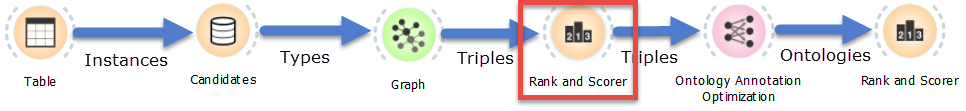
\includegraphics[width=10cm]{images/diagrams-rank-scorer.png}
		%\caption{\label{fig:your-figure2} TableMiner design by Z.Zhang}
	\end{figure}
\end{frame}
\begin{frame}{Methodology: Ranking Triples - 2}
	\begin{textblock*}{4cm}(8.5cm,0.05cm) % {block width} (coords)
		
\includegraphics[width=4cm]{images/header-rank-triples.png}
	\end{textblock*}
	\begin{definition}[Triples Ranker]
		a score is set given a condition
	\end{definition}
\end{frame}
\begin{frame}{Methodology: Ranking Triples - 3}
	\begin{textblock*}{4cm}(8.5cm,0.05cm) % {block width} (coords)
		
\includegraphics[width=4cm]{images/header-rank-triples.png}
	\end{textblock*}
	State-of-the-Art
	\begin{itemize}
		\item L2R (Learn to rank) TermPicker
	\end{itemize}
\end{frame}
\begin{frame}{Methodology: Ranking Triples - 4}
	\begin{textblock*}{4cm}(8.5cm,0.05cm) % {block width} (coords)
		
\includegraphics[width=4cm]{images/header-rank-triples.png}
	\end{textblock*}
	Scoring
	\begin{itemize}
		\item subject indicator scorer
		\item ABSTAT on frequency usage
	\end{itemize}
\end{frame}


\begin{frame}{Methodology: Making Ontologies}
	\begin{textblock*}{4cm}(8.5cm,0.05cm) % {block width} (coords)
		
\includegraphics[width=4cm]{images/header-opt.png}
	\end{textblock*}
	\begin{figure}
		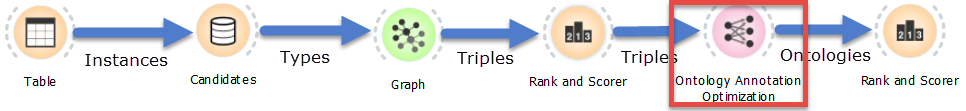
\includegraphics[width=10cm]{images/diagrams-opt.png}
		\caption{\label{fig:your-figure2} TableMiner design by Z.Zhang}
	\end{figure}
\end{frame}
\begin{frame}{Methodology: Making Ontologies}
	\begin{textblock*}{4cm}(8.5cm,0.05cm) % {block width} (coords)
		
\includegraphics[width=4cm]{images/header-opt.png}
	\end{textblock*}
	\begin{definition}[Optimizer]
		Find the path that maximize the path
	\end{definition}
\end{frame}
\begin{frame}{Methodology: Making Ontologies}
	\begin{textblock*}{4cm}(8.5cm,0.05cm) % {block width} (coords)
		
\includegraphics[width=4cm]{images/header-opt.png}
	\end{textblock*}
	State-of-the-Art
	\begin{itemize}
		\item 
	\end{itemize}
\end{frame}
\begin{frame}{Methodology: Making Ontologies}
	\begin{textblock*}{4cm}(8.5cm,0.05cm) % {block width} (coords)
		
\includegraphics[width=4cm]{images/header-opt.png}
	\end{textblock*}
	Minimum Spanning Tree
\end{frame}


\begin{frame}{Methodology: Ranking Ontologies}
	\begin{textblock*}{4cm}(8.5cm,0.05cm) % {block width} (coords)
		
\includegraphics[width=4cm]{images/header-rank-ontologies.png}
	\end{textblock*}
	\begin{figure}
		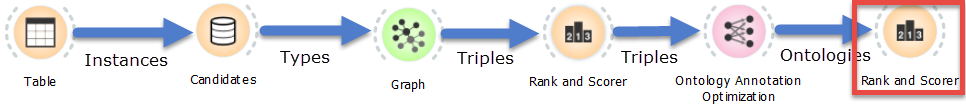
\includegraphics[width=10cm]{images/diagrams-rank-ontologies.png}
		\caption{\label{fig:your-figure2} TableMiner design by Z.Zhang}
	\end{figure}
\end{frame}
\begin{frame}{Methodology: Ranking Ontologies}
	\begin{textblock*}{4cm}(8.5cm,0.05cm) % {block width} (coords)
		
\includegraphics[width=4cm]{images/header-rank-ontologies.png}
	\end{textblock*}
	\begin{definition}[Ontologies Scorer]
		scoring ontologies due to the mapping on other ontologies
	\end{definition}
\end{frame}
\begin{frame}{Methodology: Ranking Ontologies}
	\begin{textblock*}{4cm}(8.5cm,0.05cm) % {block width} (coords)
		
\includegraphics[width=4cm]{images/header-rank-ontologies.png}
	\end{textblock*}
	State-of-the-Art
	\begin{itemize}
		\item boh!
	\end{itemize}
\end{frame}
\begin{frame}{Methodology: Ranking Ontologies}
	\begin{textblock*}{4cm}(8.5cm,0.05cm) % {block width} (coords)
		
\includegraphics[width=4cm]{images/header-rank-ontologies.png}
	\end{textblock*}
	Scoring
	\begin{itemize}
		\item the group that is more closer between the types of each possible ontology
		\item the number of ontologies that depends the result ontology
	\end{itemize}
\end{frame}


\begin{frame}{Methodology: Result}
	\begin{textblock*}{4cm}(8.5cm,0.05cm) % {block width} (coords)
		
\includegraphics[width=4cm]{images/header.png}
	\end{textblock*}
\end{frame}
\begin{frame}{Methodology: Result}
	\begin{textblock*}{4cm}(8.5cm,0.05cm) % {block width} (coords)
		
\includegraphics[width=4cm]{images/header.png}
	\end{textblock*}
\end{frame}


\begin{frame}{Introduction: }
	\begin{figure}
		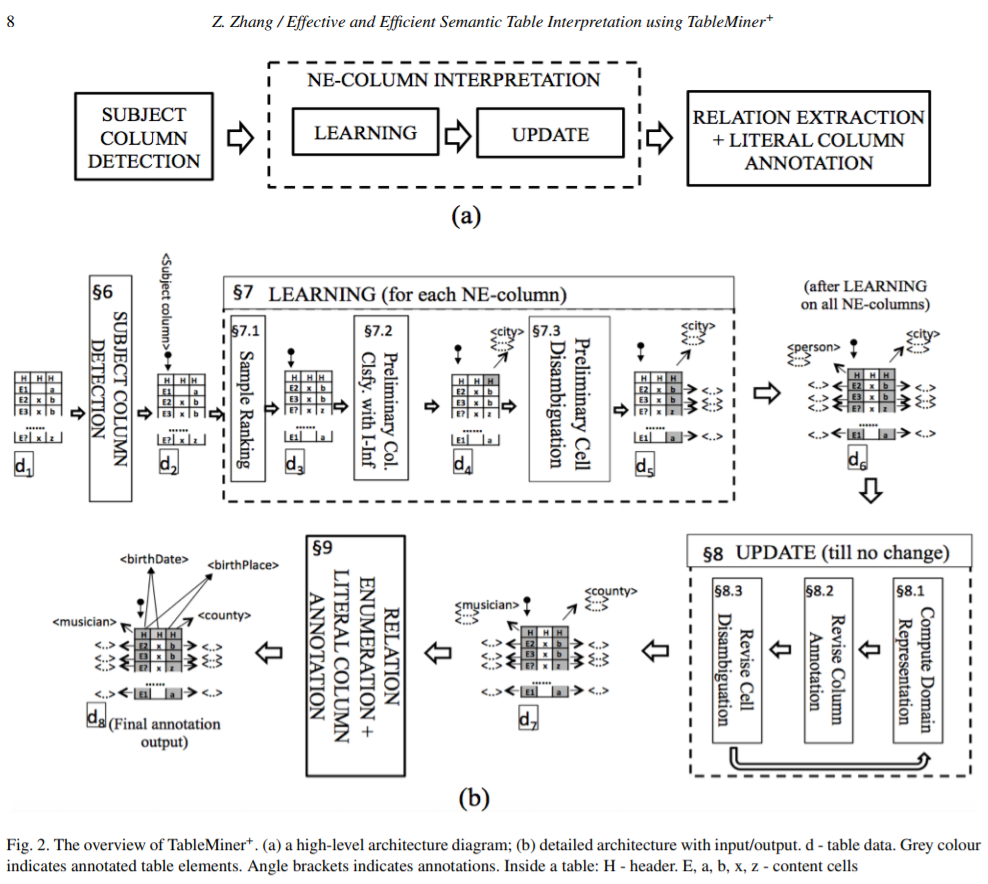
\includegraphics[width=8cm]{images/TableMiner.png}
		\caption{\label{fig:your-figure2} TableMiner design by Z.Zhang}
	\end{figure}
\end{frame}



\begin{frame}{Introduction}
	\begin{itemize}
		\item Query Input
		\item Recommender of Vocabulary Term
		      \begin{itemize}
			      \item Features for ranking
			      \item Learning to Ranking
		      \end{itemize}
		\item Query Output
	\end{itemize}
	\begin{figure}
		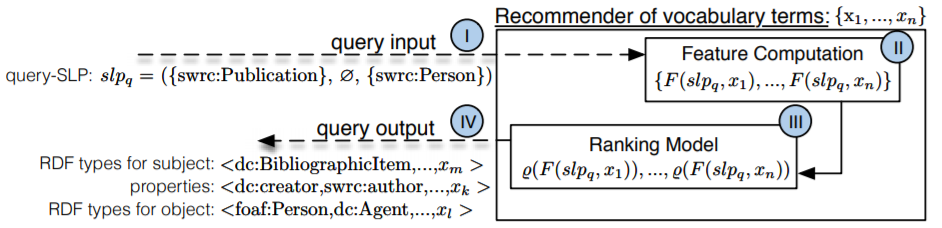
\includegraphics[width=8cm]{images/schema-queryinput.png}
		\caption{\label{fig:your-figure1}Schema of the process of the query}
	\end{figure}
\end{frame}

\begin{frame}{Introduction}
	%   \begin{itemize}
	%     \item The study that is taken as a reference is “Mapas de Pobreza en Guatemala al 2002” by the National Institute of statistics (INE) of Guatemala. 
	%     \item In this study the poverty is taken as a generalized poverty, which take into account the living standard of a person.
	%     \item url: \url{http://fadep.org/wp-content/uploads/2016/10/D-5_MAPAS_DE_POBREZA_GUA_2002.pdf}
	%   \end{itemize}
\end{frame}

\begin{frame}{Introduction}
	%   \begin{figure}
	% 		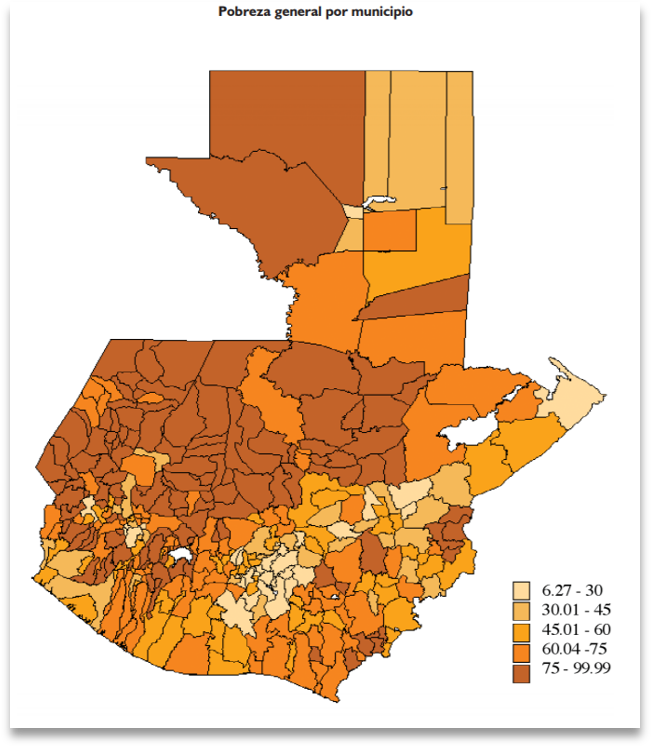
\includegraphics[width=5cm]{images/fig3-map.png}
	% 		\caption{\label{fig:your-figure3}Guatemala State Map with a color scale of the generalized poverty}
	% 	\end{figure}
\end{frame}

\begin{frame}{Dataset ABSTAT and ontologies}
	% \begin{itemize}
	% 	\item The Data is define in tree modules, the living conditions at the residence, the conditions of each house/apartment/room inside the residence, and finally the characteristics of each person that lives in each residence.
	% \end{itemize}
	% \begin{figure}
	% 	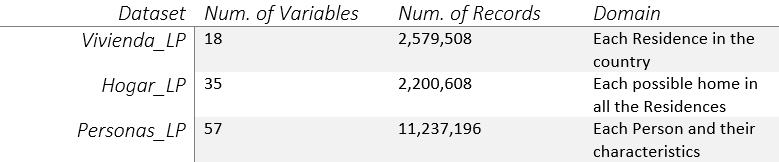
\includegraphics[width=9cm]{images/alldataset.png}
	% 	\caption{\label{fig:alldataset}Datasets taking into consideration in order to make the analysis}
	% \end{figure}
	% \begin{figure}
	% 	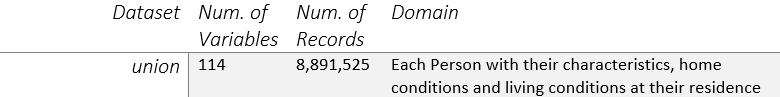
\includegraphics[width=9cm]{images/uniondataset.png}
	% 	\caption{\label{fig:uniondataset}Resulting dataset of the union of Vivienda\_LP, Hogar\_LP and Personas\_LP; filtering records}
	% \end{figure}
\end{frame}


%%%%%%%%%%%%%%%%%%%%%%%%%%%%%%%%%%EXTRA%%%%%%%%%%%%%%%%%%%%%%%%%%%%%%%%%%%%%%%%%

% \begin{frame}{Poverty Index Creation: MPI Aspects }
% 	\begin{itemize}
% 		\item The variables of the Datasets has been measured and has been grouped by the aspects of the MPI of Oxford.
% 	\end{itemize}
% 	\begin{figure}
% 		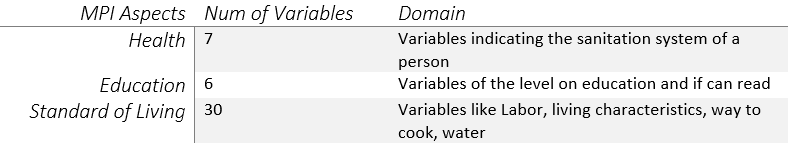
\includegraphics[width=9cm]{images/indexvariables.png}
% 		\caption{\label{fig:indexvariables}Variables took into consideration by the aspects of the MPI created, and the characteristics that the variables have}
% 	\end{figure}
% \end{frame}

% \begin{frame}{Poverty Index Creation: Filtering}
% 	\begin{itemize}
% 		\item Each Variable taken into consideration has effects on the selected data and this lead to some records to be non applicable.
% 		\begin{itemize}
% 			\item Health - the selected data requires that the residence is actually being inhabited by a person and is not a store 
% 			\item Education - the selected data requires that the person been interviewed has more than 6 years old
% 			\item Living - all the persons that satisfy the requirements of Health and Education have the living data
% 		\end{itemize}
% 	\end{itemize}
% \end{frame}

% \begin{frame}{Poverty Index Creation: Result}
% 	\begin{itemize}
% 		\item The resulting dataset has been done by filtering only the variables that were involved on the Multidimensional Poverty Index (MPI) created, and filtering only the records that applied to MPI variables.
% 	\end{itemize}
% 	\begin{figure}
% 		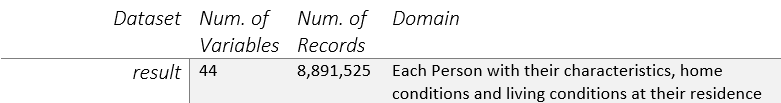
\includegraphics[width=9cm]{images/resultdataset.png}
% 		\caption{\label{fig:resultdataset}Resulting dataset of the union of Vivienda\_LP, Hogar\_LP and Personas\_LP; filtering variables and records}
% 	\end{figure}
% \end{frame}

% \begin{frame}{Poverty Index Comparison - 1}
%   \begin{itemize}
%     \item The metric that it takes as comparison is the index general poverty of the Guatemalan study by INE, that also seek to measure the poverty not only by the income but by the aspects of living of a person. 
%   \end{itemize}
% \end{frame}


% \begin{frame}{Poverty Index Comparison - 2}
%   \begin{figure}
% 		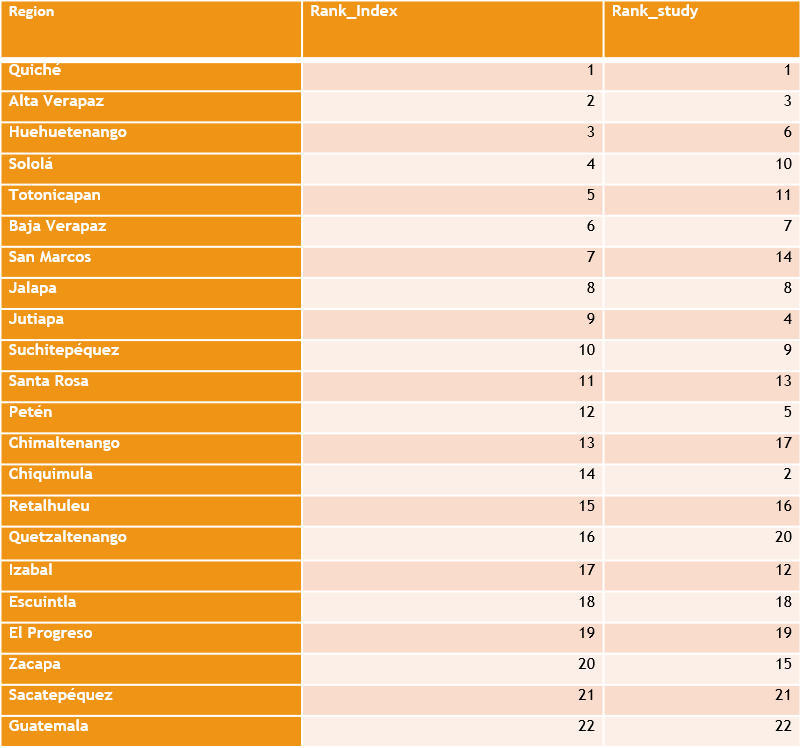
\includegraphics[width=6.5cm]{images/fig4-IndexComp.png}
% 		\caption{\label{fig:your-figure4}Index Table comparison, where Rank\_index is the rank of the generated index with the MPI metrics. The Rank\_study is the rank of the index of Generalized Poverty by the Guatemala Study}
% 	\end{figure}
% \end{frame}

% \begin{frame}{Poverty Index Comparison - 3}
%   \begin{itemize}
%     \item The comparison was made with the paired difference test of “Wilcoxon Signed-Rank Test”.
%     \item The result is that the null hypothesis can’t be refuted, where H0: is that the difference between the pairs follows a symmetric distribution around zero, whit a 0.05 of significance level. With a p-value = 0.8155. So we can't prove that they are different, making a well comparison of the index.
%   \end{itemize}
% \end{frame}

% \begin{frame}{Classification Trees: Introducction - 1}
% 	\begin{figure}
% 		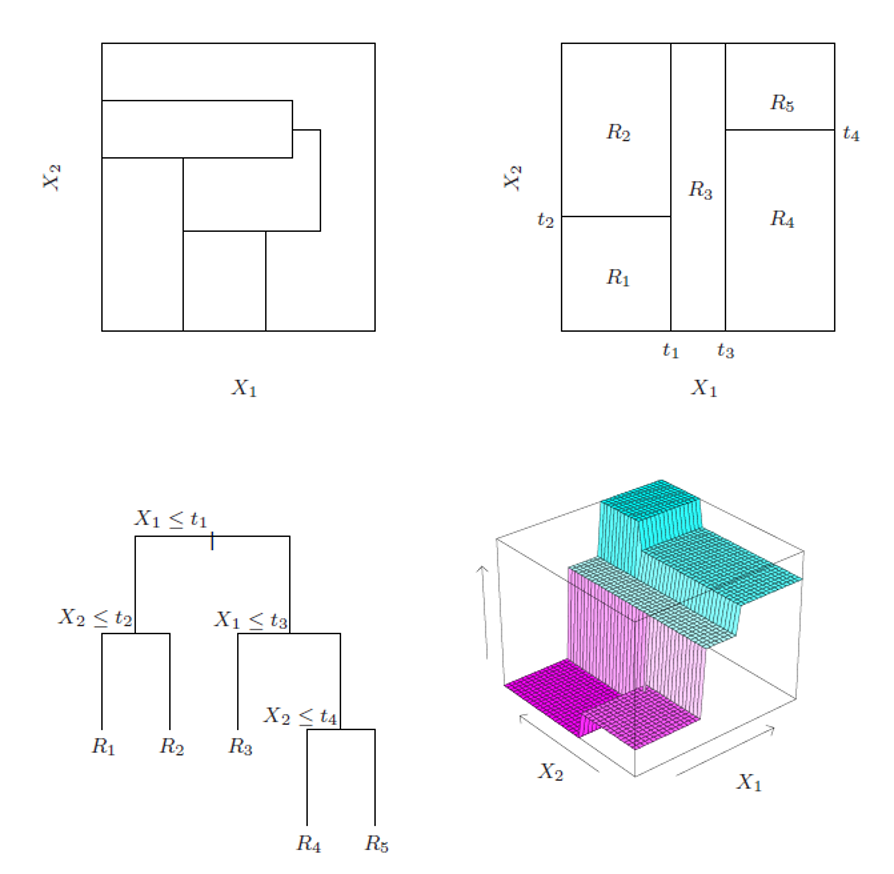
\includegraphics[width=5cm]{images/fig5-decisiontrees.png}
% 		\caption{\label{fig:dtintro} Rerpresents graphicly the regions of a classification tree}
% 	\end{figure}
% \end{frame}

% \begin{frame}{Classification Trees: Introducction - 2}\Fontvi
% 	$$\begin{array}{c}$$
% 	{Getting\ as\ a\ response\ variable\ Y\ and\ p\ explicative\ variables\ as\ X\ }\\{the\ target\ categorical\ variable\ taken\ into\ consideration\ is\ poverty}
% 	\\
% 	{where\ (x_i,y_i)\ goes\ with\ i = 1,2,...,N\ and\ x_i = (x_{i1},x_{i2},...,x_{ip}),\ giving\ N=2\ and\ p=43}\\
% 	{letting\ be\ k\ as\ each\ class\ of\ the\ target\ variable\ and\ m\ as\ identifier\ of\ each\ node.}\\
% 	{In\ a\ node\ m,\ representing\ R_m\ as\ the\ Region}\\
% 	{N_m\ representing\ the\ quantity\ of\ observations\ in\ m}\\\\\\
% 	{It\ can\ be\ said\ that\ the\ proportions\ between\ each\ class\ k\ of}{the\ target\ variable\ in\ each\ node\ m\ can\ be\ represented\ as:}\\
% 	$$
% 		\hat{p}_{mk} = \frac{1}{N_m} ∑_{x_i∈R_m}I(\,y_i = k)\,
% 	\end{array}
% 	$$
% \end{frame}

% \begin{frame}{Classification Trees: Introducction - 3}\Fontvi
% 	$$
% 	\begin{array}{c}
% 	$${the\ splitting\ rule\ took\ was\ the\ Missclassification\ Error,\ where\ can\ be:}\\$$
% 	$${Missclassification\ error:}$$\\
% 	$${Gini\ index: }$$\\
% 	$${Cross-entropy\ of\ deviance:}$$
% 	\end{array}
% 	\begin{array}{c}
% 		\frac{1}{N_m} 		
% 			∑_{i∈R_m}I(\,y_i≠k(\,m)\,)\,  =
% 			1-\hat{p}_{mk(\,m)\,};
% 		$$\\$$
% 			∑_{k≠k'}\hat{p}_{mk}\hat{p}_{mk'} =
% 			∑_{k=1}^{K}\hat{p}_{mk}(\,1-\hat{p}_{mk})\,;
% 		$$\\$$
% 		-∑_{k=1}^K\hat{p}_{mk}\log\hat{p}_{mk};
% 	\end{array}
% 	$$
% \end{frame}



% \begin{frame}{Classification Trees: Introducction - 2}
% 	\begin{figure}
% 		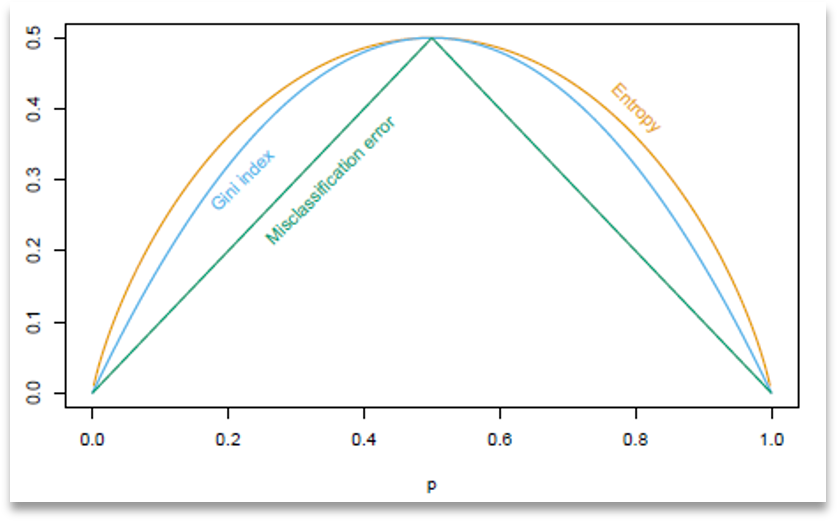
\includegraphics[width=5cm]{images/fig6-dtimpurity.png}
% 		\caption{\label{fig:} Shows the different spliting rules of the classification tree by the measure of impurity, in the x axis show the proportions of the binary target.}
% 	\end{figure}
% \end{frame}


% \begin{frame}{Classification Trees: Result - 1}
% 	\begin{figure}
% 		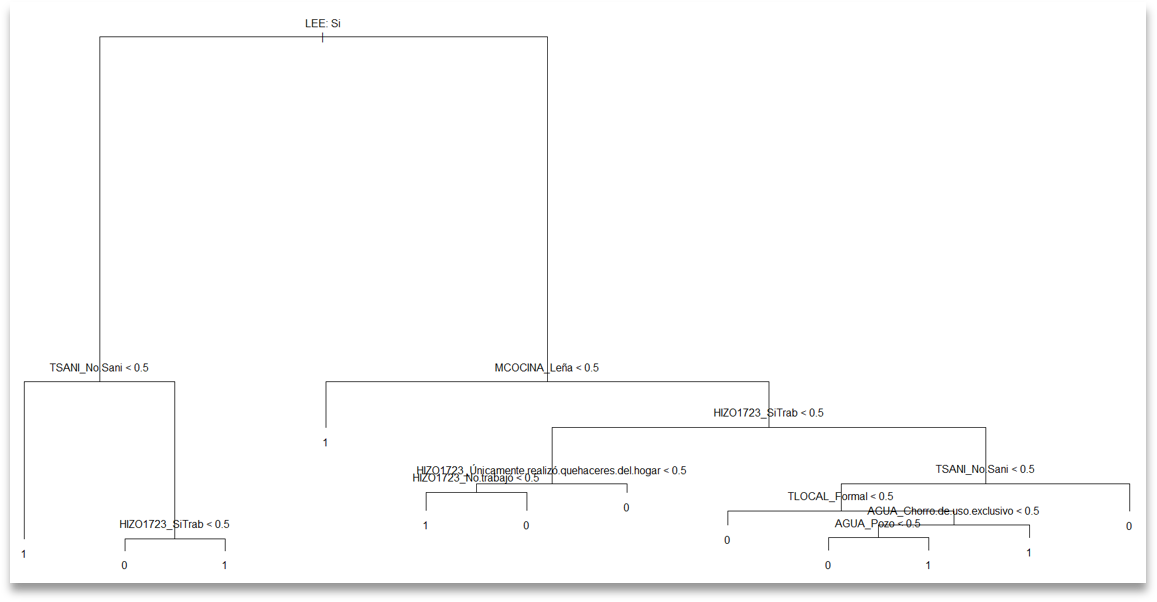
\includegraphics[width=10cm]{images/fig7-dtresult.png}
% 		\caption{\label{fig:dtresult} show the resultant tree of the dichotomous target variable  and the most significant variables}
% 	\end{figure}
% \end{frame}


% \begin{frame}{Classification Trees: Result - 2}
% 	\begin{figure}
% 		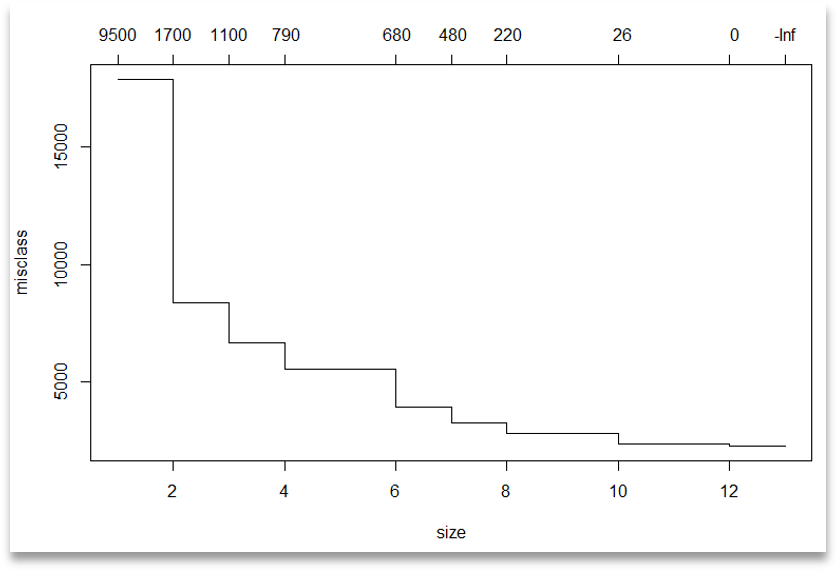
\includegraphics[width=8cm]{images/fig8-dtmissclas.png}
% 		\caption{\label{fig:dtmissclas} Missclassification rate of the prediction by the resultant model of the training of the Classification tree}
% 	\end{figure}
% \end{frame}


% \begin{frame}{LDA (Linear Discrimant Analysis): Introducction - 1}
% 	\begin{figure}
% 		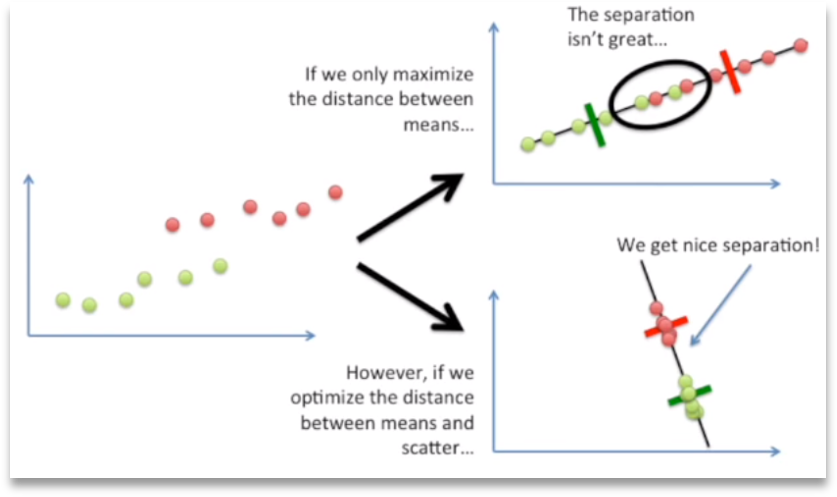
\includegraphics[width=8cm]{images/ldaintro.png}
% 		\caption{\label{fig:ldaintro} The Linear Discriminant Analysis tray to maximize the eucledean distance between groups separation and minimize the variation of each group}
% 	\end{figure}
% \end{frame}

% \begin{frame}{LDA: Introduction - 2}\Fontvi
% 	$$
% 	\begin{array}{c}
% 		$$
% 		{Given\ f_k(x)\ the\ class-conditional\ density\\\ of\ X\ in\ class\ G=k\ and\ letting\ \pi_k\ be\ the\ prior\ probability\ of\ class\ k,\\
% 		Supposing\ that\ each\ class\ density\ is\ modeled\\\ by\ a\ multivariate\ Gaussian,\ the\ discriminant\ function\ is:}\\
% 		$$
% 		\delta_k(x)=x^T∑^{-1}\mu_k-\frac{1}{2}\mu_k^T∑^{-1}\mu_k+\log\pi_k;
% 		$$\\
% 		$$
% 		\hat{ \pi }_k=\frac{N_k}{N},\ where\ N_k\ is\ the\ number\ of\ class-k\ observations;
% 		$$\\
% 		$$
% 		\hat{\mu}_k = ∑_{g_i = k}x_i/N_k
% 		$$\\
% 		$$ 
% 		$$\\{supposing\ that:}
% 		$$
% 		∑_k=∑∀k;
% 		$${where\ the\ target\ variable\ poverty\ is\ categorical\ having\ 2\ classes,\ 0\ or\ 1}\\
% 		$$
% 	\end{array}
% 	$$
% \end{frame}


% \begin{frame}{LDA: Result - 1}
% 	\begin{figure}
% 		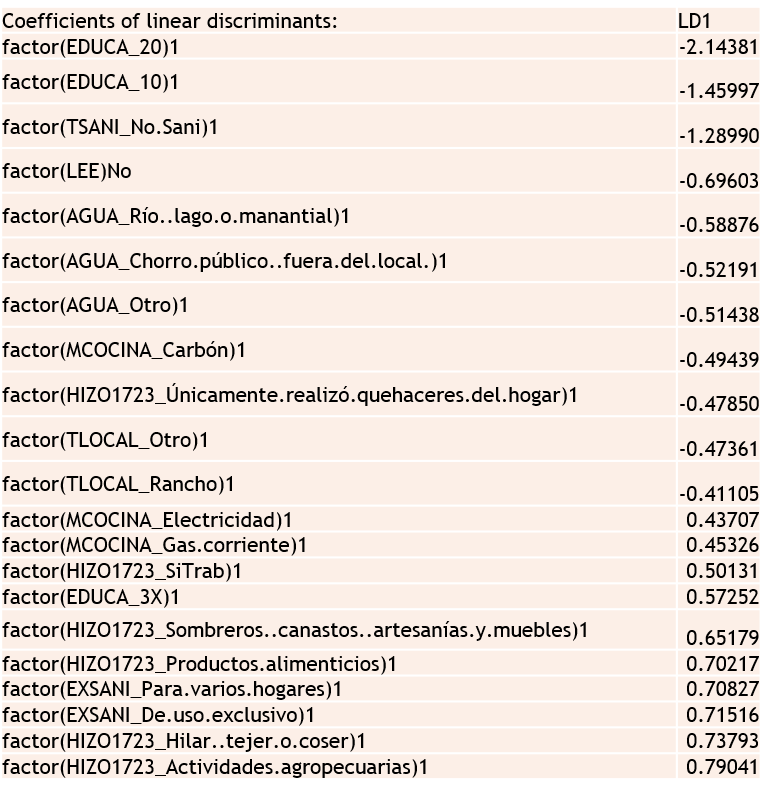
\includegraphics[width=6cm]{images/ldamostvars.png}
% 		\caption{\label{fig:ldamostvars} The most significant variables that separate better the groups if a person is poor or not}
% 	\end{figure}
% \end{frame}



% \begin{frame}{LDA: Result - 2}
% 	\begin{figure}
% 		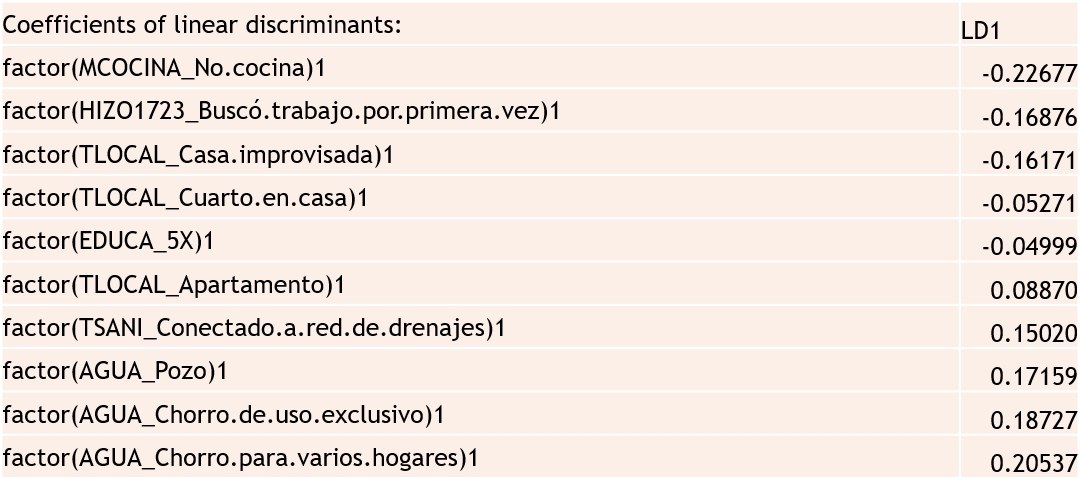
\includegraphics[width=7cm]{images/ldalessvar.png}
% 		\caption{\label{fig:ldalessvar} The less significant variables that separate better the groups if a person is poor or not}
% 	\end{figure}
% \end{frame}



% \begin{frame}{LDA: Result - 3}
% 	\begin{figure}
% 		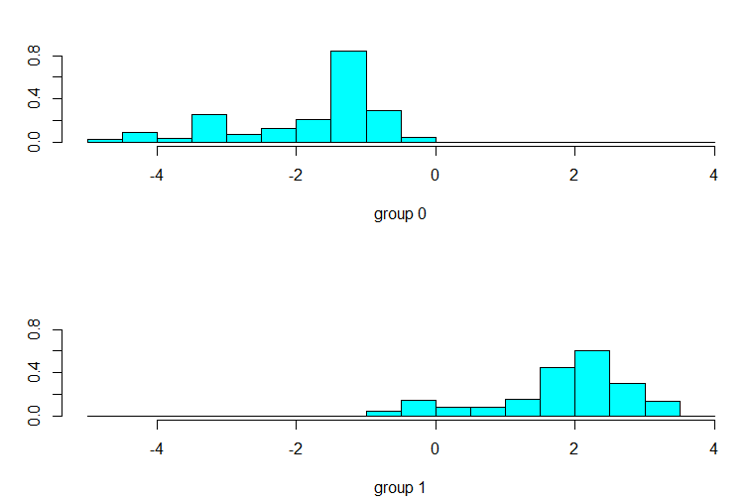
\includegraphics[width=8cm]{images/ldaresult.png}
% 		\caption{\label{fig:ldaresult} Histogram of the quantity of variables that separate each group, the group 0 determines if a person is poor and the group 1 if not}
% 	\end{figure}
% \end{frame}

\begin{frame}
	\frametitle{the scope}
	\begin{itemize}
		\item adesso faccio i 
		\item sdfkjljs
		\item lasjdfjlasdf
		\item lajsdfkjas
		\item 
	\end{itemize}
\end{frame}



\begin{frame}{Conclusion}
	\begin{itemize}
		\item
	\end{itemize}
\end{frame}

\begin{frame}{Reference}
	\begin{itemize}
		\item SPARQL types
		\item LOD TermPicker
		\item LOV (others)
		\item ABSTAT
		\item TableMiner
	\end{itemize}
\end{frame}



\end{document}
